
\documentclass[sigconf,authorversion,nonacm]{acmart}

\usepackage{multirow}
\usepackage[symbol]{footmisc}
\renewcommand{\thefootnote}{\fnsymbol{footnote}}
\usepackage{caption}

\begin{document}

\title{Feature Extraction from Customer Reviews for Amazon Recommender System}

\author{Group 19 - Candidate numbers: 42193, 44326, 52208}

\begin{abstract}
  The study focuses on comparing the overall performance of various customer-review-based recommender systems on the Amazon Product Reviews dataset, by evaluating models on both their ability to make rating predictions and computational performance. Two recommender systems that incorporate customer reviews to make predictions were constructed with guidance from literature, and compared against two benchmark models that only utilise product ratings. The two customer-reviews-based recommender models use natural language processing techniques such as Word2Vec and Term Frequency-Inverse Document Frequency (TF-IDF) to extract information about product suitability for a customer. We found that although a simple baseline model performs the best with an average MSE of 1.58 across categories, it is only marginally better than our general-setting Similarity-Rating model (MSE = 1.78), which compares how similar a customer's previous reviews are with reviews written by other customers for an unseen product to compute the most plausible rating. This study also explores the distributed computing gains from using big data analysis systems such as the Google Cloud Platform, Apache Hadoop and Apache Spark, and compared performance across models with different data partitioning systems. It was found that most models benefitted from increasing partitions up to a certain optimal setting, and the Baseline Rating Model had the best computation time for all partition settings compared to other models.

\end{abstract}

\keywords{Recommender systems, Word2Vec, Term Frequency-Inverse Document Frequency, Distributed Computing}

\settopmatter{printfolios=true}
\maketitle

\section{Introduction}
    Recommender systems can largely been categorised into two main categories, content-based recommender systems and collaborative filtering recommender systems. Content-based recommender systems recommend items which are similar to items the customer has purchased in the past\cite{Pazzani2007}. Collaborative filtering recommendation systems exploit the similarity between users to recommend items which have been chosen by similar users\cite{Factor10}. User ratings and customer reviews are the main sources of data used in these systems. 
    
    E-commerce recommender systems have achieved significant success in the marketplace and they are arguably paramount to an e-commerce platform's success. Amazon is one of the largest large e-commerce platforms in the world. It applies data mining techniques on user behaviour data by analysing what users have browsed, purchased and reviewed, and compares it with what similar users are doing\cite{krysik_2021}. The insights gained are fed into a recommender system. This recommender system provides a personalised shopping experience for such users and has become one of Amazon's core competencies over that of other e-commerce platforms. These systems not only reduce information overload but also contribute to increasing sales, improving customer satisfaction and enhancing brand loyalty by offering insights into the preferences of users and the quality of products. 

    Customer reviews have been incorporated into recommender systems to create review-based rating prediction systems. This study focuses on comparing and contrasting the performance of multiple rating prediction systems on the Amazon Review dataset. The computational complexity of applying these systems on large datasets is a challenge. The proposed scheme in this study focuses on scaling these systems by using distributed computing techniques such as Apache Hadoop and Apache Spark, and big data analysis platforms such as the Google Cloud Platform. The study also illustrates computational gains in model performance from applying distributed computing techniques through numerical experiments. 
    
\section{Related work}
    We reviewed the literature for work on creating recommender systems and found that while there is a vast amount of literature on building recommender systems based on product ratings, building recommender systems based on customer reviews text is relatively less established. Many of these research also focus on explaining one major model with some variations in great detail, with less focus on comparison with other types of models. In addition, very few of these papers detail both distributed computing methods used for scaling models and also investigate the impact of different distributed computing settings on model performance, even though this is a crucial part of running a large recommender model. Consequently, we think there is room for us to improve on the existing literature by 1. comparing across more different types of models for customer reviews-based recommender systems and 2. providing more details and insights on distributed computing methods for scaling similar models. 

    There were a number of methods trialled in the literature for using text from customer reviews to build recommender systems. Some of the systems combined customer reviews text with ratings for the predictions, while others just used customer reviews text. From our research, we found that the methods trialled can be broadly grouped into three categories: similarity-based methods, sentiment-based methods and topic modelling-based methods. 

    Similarity-based methods generally compare the similarity of existing reviews by a customer and existing reviews of a product they have never seen before to predict whether a customer would be interested in the product. This is predominantly done by transforming reviews into word embedding representation, which can then be translated into similarity scores across reviews. This was done in \cite{hasanzadeh2022based}, which used Word2Vec for the word embeddings. Their method also combines the helpfulness voting score in an attempt to mitigate prediction inaccuracies caused by inaccurate review ratings. 

    Sentiment-based methods extract the sentiment of reviews for a product to predict whether a customer would enjoy a product or not. This is sometimes combined by extracting features from customer reviews to determine what features a customer is interested in, and getting the sentiment of the feature mentions for reviews of a particular product. This was the general method used by \cite{d2017exploiting}, where they extracted features from customer reviews with heuristics and other natural language processing techniques. 

    Topic-modelling-based methods are similar to sentiment-based methods in that it extracts features from reviews, but does it by using neural networks and learning a higher-level feature which may be a combination of multiple features in sentiment-based methods. These are also often combined with a model based on matrix factorization for ratings to use customer reviews to supplement a basic rating-based prediction model. An early paper which proposed this method did this and found significant improvements in performance \cite{mcauley2013hidden}. A later paper improves on this model and proposes a model that can take in additional features on top of the extracted LDA features \cite{aslanyan2021utilizing}.

    Due to time and resource constraints, the scope of the project was narrowed to focus on similarity-based methods and sentiment-based methods. The various methods from other research detailed above helped inform the final algorithms we use, which are streamlined versions of a general similarity-based and sentiment-based method. Although we do not extend beyond the models that have already been proposed in the literature, we contribute by drawing comparisons across more different models and providing further insights on running the model with distributed computing methods. 

\section{Methodology}

This section details the methodology of our project. We first introduce the dataset used and the four models that we focus on. Then, we detail the methodology for the two main investigations of our project: first, drawing cross-model comparisons and second, demonstrating distributed computing gains and changes from changing data partitions of our model. We focus on changing partitions as it is one of the most straightforward distributed computing techniques yet has a huge potential for computational gains. Finally, we discuss other distributed computing techniques we utilised throughout the project.

\subsection{Data}
    The dataset used in this study is the \href{https://cseweb.ucsd.edu/~jmcauley/datasets/amazon_v2/}{Amazon review dataset} updated in 2018 and made available by Jianmo Ni from UCSD. This dataset comprises over 233.1 million reviews from Amazon.com, spanning from May 1996 to October 2018 \cite{ni_li_mcauley_2019}. It is chosen for its completeness, good documentation, and because of Amazon's domineering position in the e-commerce market. The compressed file size for all reviews is 34GB, making analysing customer reviews from this dataset a task that demands the use of distributed computing methods. For the specific implementation of the study, we utilized the per-category data, which contains review data for each category, and includes the following information:
    
    \begin{itemize}
    \item \verb|reviewerID|: ID of the reviewer
    \item \verb|asin|: ID of the product
    \item \verb|reviewerName|: name of the reviewer
    \item \verb|vote|: number of helpful votes for the review
    \item \verb|style|: a dictionary of the product metadata
    \item \verb|reviewText|: text of the review
    \item \verb|overall|: rating of the product made by reviewer
    \item \verb|summary|: summary of the review
    \item \verb|unixReviewTime|: unix time of the review
    \item \verb|reviewTime|: time of the review
    \item \verb|image|: link of image attached to the review
    \end{itemize}
    
    Due to the computational constraints of a standard Google Cloud Platform account and the limited timeframe of the project, we faced difficulties in running models through all datasets. A total number of 19 per-category datasets were examined ultimately, where we started from the smallest datasets and ran our models through increasingly larger datasets. The datasets used are bolded in Table 1. 
    
    We split each of the datasets into two datasets prior to running the models: training and test data, by randomly choosing $80\%$ of each dataset as the training data and the remaining $20\%$ as the test data. The number of observations and file size of the per-category data used in this study are shown in Table~\ref{tab:stat}. Then, we train each model on the testing data and evaluate the corresponding predictions using test data. The subset of (\verb|asin|, \verb|reviewerID|, \verb|overall|) for the Baseline Rating Model and Alternating Least Square (ALS) model, and (\verb|asin|, \verb|reviewerID|, \verb|overall|, \verb|reviewText|) for the Similarity-Rating Model and Sentiment-Feature Model.

    \begin{table}
        \caption{Statistics of Per-category Data}
        \label{tab:stat}
        \begin{tabular}{lrr}
        \toprule
        \textbf{Dataset} & \textbf{Reviews} & \textbf{Size} \\
        \midrule
        \textbf{All Beauty} & 371,345 & 45M \\
        \textbf{Amazon Fashion} & 883,636 & 89M \\
        \textbf{Appliances} & 602,777 & 66M \\
        \textbf{Arts Crafts and Sewing} & 2,875,917 & 292M \\
        Automotive & 7,990,166 & 866M \\
        Books & 51,311,621 &  11G\\
        \textbf{CDs and Vinyl} & 4,543,369 & 1.1G \\
        Cell Phones and Accessories & 10,063,255 & 1.1G  \\
        Clothing Shoes and Jewelry & 32,292,099 &  3.3G \\
        \textbf{Digital Music} & 1,584,082 & 207M \\
        Electronics & 20,994,353 & 3.1G \\
        \textbf{Gift Cards} & 147,194 & 11M \\
        \textbf{Grocery and Gourmet Food} & 5,074,160 & 560M \\
        Home and Kitchen & 21,928,568 & 2.6G  \\
        \textbf{Industrial and Scientific} & 1,758,333 & 201M \\
        \textbf{Kindle Store} & 5,722,988 & 1.1G \\
        \textbf{Luxury Beauty} & 574,628 & 70M \\
        \textbf{Magazine Subscriptions} & 89,689 & 12M \\
        Movies and TV & 8,765,568 & 1.4G \\
        \textbf{Musical Instruments} & 1,512,530 & 222M \\
        \textbf{Office Products} & 5,581,313 & 666M \\
        \textbf{Patio Lawn and Garden} & 5,236,058 & 640M \\
        \textbf{Pet Supplies} & 6,542,483 & 860M \\
        \textbf{Prime Pantry} & 471,614 & 43M \\
        \textbf{Software} & 459,436 & 94M \\
        Sports and Outdoors & 12,980,837 & 1.6G \\
        Tools and Home Improvement & 9,015,203 & 1.1G \\
        Toys and Games & 8,201,231 & 953M \\
        \textbf{Video Games} & 2,565,349 & 499M \\ \midrule
         \multicolumn{3}{l}{\textit{Note:} Datasets in bold text were used in the study.} \\ \bottomrule
        \end{tabular}
    \end{table}


\subsection{Models}
This section introduces and outlines the models we used to generate rating predictions for a given reviewer and product pair. We compare four models in total, with two being baseline models with no customer reviews and the other two being models with customer reviews inspired by literature. We use two baseline models because although ALS is well established as a sparse matrix factorisation method for designing recommender systems, it is still somewhat computationally costly, and we thought it would be interesting to compare its performance with an even more simple baseline model. We propose two models Similarity-Rating and Sentiment-Feature, which are essentially general models for similarity-based and sentiment-based methods observed in the literature, which we believe will yield interesting comparison results.

Each model is an algorithm that takes in a \verb|reviewerID| and \verb|productID|, then outputs a predicted \verb|rating|. The algorithms use information from a training dataset to generate the predictions, where two of the models only consider known ratings for the predictions, and another two models consider the text from customer reviews as well. 

\subsubsection{Baseline Rating Model (No Customer Reviews)}
    The baseline rating model acts as a simple baseline by making rating predictions based only on other known ratings, namely with an average rating across all reviews and mean ratings for a given reviewer and product pair. It is best summarised by the equation $$ \hat{r}_{up} = \alpha + \bar{r}_u + \bar{r}_p $$ $\alpha$ refers to the average rating across all reviews in a category, $\bar{r}_u$ refers to the difference between $\alpha$ and mean rating of all reviews for reviewer (user) $u$, and similar for product $p$ with $\bar{r}_p$. \cite{aslanyan2021utilizing} 

\subsubsection{Alternating Least Squares Model (No Customer Reviews)}

    The Alternating Least Square (ALS) model was also implemented as a baseline by predicting overall ratings given by reviewers and products. The model factorises the reviewer-product matrix, denoted by $r_{ui}$, which is factorized into two lower-dimensional matrices, known as latent factor matrices.

    In our specific implementation, we chose to decompose the original matrix into 10 latent factors. These factors are represented as two matrices: the reviewer-feature matrix $x_{u}$ and the product-feature matrix $y_{i}$. Hence, we have the approximation:
    $$r_{ui} \approx x_u^T y_i$$
    
    The next step involves an iterative algorithm designed to optimize the latent factor weights by alternating between fixing $x_u$ as constant and optimizing $y_i$ as convex, and fixing $y_i$ as constant and optimizing $x_u$ as convex with a maximum of 15 iterations. The alternating steps allow the algorithm to converge to the minimum least squares error between predicted and actual ratings, which can be formulated as
    $${\operatorname{argmin}} \sum_{r_{ui}} (r_{ui} - x_u^T y_i)^2 + \lambda \left(\sum_u ||x_u||^2 + \sum_i ||y_i||^2 \right)\cite{Gosh21}$$ where we chose the regularization factor $\lambda$ to be 0.2 to avoid overfitting, and also to ensure consistency across all datasets in our evaluation, enabling a fair comparison of the performance of algorithms. 
    
\subsubsection{Similarity-Rating Model (With Customer Reviews)}

The similarity -Rating method aims to compare previous customer reviews by a reviewer with customer reviews written by other customers for a product to find the most likely rating a reviewer will give a product they have not reviewed before. This is done by converting the customer reviews into a Word2Vec representation and computing a cosine similarity score. It is inspired by \cite{hasanzadeh2022based}, though we take a more general approach than them. 

We first train a Word2Vec model by taking all the reviews in the training dataset as our corpus. Word2Vec aims to generate a vector representation of a word by considering the relationship of the word with others within a corpus. Training a Word2Vec Model separately on the corpus of customer reviews has multiple advantages over loading a pretrained Word2Vec model: 1. A vector representation can be obtained for all of the words on the corpus, 2. It should learn the relationship for category-specific jargon words better and 3. The model is of a smaller size and is thus more memory-efficient. 

Then, we obtain the average Word2Vec score for all the reviews for a reviewerID grouped by rating. In other words, we take all the reviews for this particular reviewer with a 1 star rating, get the Word2Vec representation for every word for each review, then take an average across all the vectors. This is repeated for 2 stars to 5 stars ratings. The whole process is then repeated by taking all the reviews for a particular productID instead of for reviewerID. In total, we end up with 10 vectors, where each vector is the average vector representation for reviews of either the targetted reviewer or the product across the 5 ratings. 
Then, we obtain the average Word2Vec score for all the reviews for a reviewerID grouped by rating. In other words, we take all the reviews for this particular reviewer with a 1 star rating, get the Word2Vec representation for every word for each review, then take an average across all the vectors. This is repeated for 2 stars to 5 stars ratings. The whole process is then repeated by taking all the reviews for a particular \verb|productID| instead of for \verb|reviewerID|. In total, we end up with 10 vectors, where each vector is the average vector representation for reviews of either the targetted reviewer or the product across the 5 ratings. 

Finally, we compute the cosine similarity score for each pair of vectors with the same rating, yielding 5 cosine similarity scores. The cosine similarity score is calculated as follows for the user (reviewer) $u$, product $p$ and rating $r$: 
$$ \cos ({\textbf{W}_{ur}}, {\textbf{W}_{pr}}) = \dfrac {\textbf{W}_{ur} \cdot \textbf{W}_{pr}} {||\textbf{W}_{ur}|| * ||\textbf{W}_{pr}||} $$
A cosine similarity score for 1-star rating could thus be interpreted as how similar the average 1-star reviews from a particular reviewer are to the average 1-star reviews for a particular product. The idea is that if the similarity score is higher, it means that the reviewer is more likely to give that rating to this unseen product. We thus then get the rating that yields the highest cosine similarity score as the predicted rating. 

The algorithm works less well when there are few reviews for either the reviewer or the product we are looking at since a cosine similarity score cannot be generated for a rating if we do not have both existing reviews at a certain rating given by the reviewer and also for the particular product. When all cosine similarity scores cannot be computed, the algorithm defaults to giving the average rating across all products for the category as the prediction. 

\subsubsection{Sentiment-Feature Model (With Customer Reviews)}

    The Sentiment Feature Model makes predictions by considering the features important to a reviewer and looking at the average sentiment of mentions of these features amongst the product of interest. The algorithm only draws on the text of customer reviews and ignores the relevant rating. This method is inspired by (citation), which also uses sentiment of features to consider whether a product should be recommended to a reviewer or not, where their method uses more heuristics. 

    First, we extract the top 3 features by looking at the corpus of words from all reviews by the reviewer of interest. The top 3 features are the words with the highest Term Frequency-Inverse Document Frequency (TF-IDF) score for the particular reviewer. TF-IDF is calculated by the following formula \cite{joachims1996probabilistic}: 

    $$ TF-IDF(f, d) = TF(f,d) \cdot IDF(f) $$
    $f$ denotes feature and $d$ denotes document, where for our model a document consists of the corpus of all reviews from a single reviewer. $TF(f,d)$ refers to term frequency of $f$ in $d$, which is the number of occurrences of feature $f$ within all the reviews from a single reviewer. $IDF(f)$ is calculated as follows: 
    
    $$ IDF(f) = log \frac{|D|}{DF(f)}$$
    $|D|$ refers to the total number of documents, which is the total number of reviewers here. $DF(f)$ is the document frequency of a feature, which is the number of reviewers that have mentioned feature $f$ at least once in at least one of their reviews. 
    
    By getting the words with the highest TF-IDF score, it is hoped that these are a good representation of what a reviewer cares for the most as they mention it frequently in past reviews and are also words that are not frequently used by other reviewers. To improve the quality of features extracted, pre-processing was performed on the corpus, which includes converting all tokens (words) to lowercase, stripping punctuation, filtering out stop words and lemmatising words where possible. 

    Subsequently, the algorithm looks at all mentions of the chosen 3 features within all reviews for the product of interest. For each of the mentions, the feature itself and the 5 words before and after the feature were extracted as a phrase. This is based on the idea that the sentiment of a review towards a particular feature may not be evident in the feature itself but can be inferred from words used around the feature. For example, a feature a reviewer might care about in beauty products is “colour”, but the word in itself is fairly neutral. If a phrase from a review says, “The makeup palette has an amazing selection of colours”, then we can utilise sentiment from words such as “amazing” to infer that this feature is mentioned positively in this product, and thus the reviewer is likely to like this product and give it a high rating. 

    We found the average sentiment of the phrase by considering the average sentiment score of each word, which was done by applying the VADER sentiment analysis tool from the natural language processing library \verb|nltk|, and averaged the found average sentiments across all phrases for all mentions of the feature. This was repeated in the three chosen features, such that we get an averaged sentiment score for mentions of each feature for this particular product from the scale -1 to +1. Finally, we added these three scores together and rescaled them linearly (multiplying the score by $\frac{2}{3}$ and adding 3) such that the scores will be on the Amazon rating scale of 1 to 5. 

\subsection{Cross-Model Comparisons}

We compared the performance of the four models across categories in the customer reviews dataset. This allowed us to also observe the differences in model performance across categories to draw better conclusions about the advantages and disadvantages of each model. 
To facilitate a fair comparison, we ensured that for the same category, each model was evaluated on its performance on the same test dataset, and also trained or extracted information from the same train dataset (from \verb|reviewText| and/or \verb|rating|). An 80-20 random split was performed on the reviews dataset for each category to achieve this as a simple rule of thumb. 

As hyperparameters were not the focus of this report, we used default parameters whenever possible and either used heuristics or referred to the literature for setting parameters. For example, the Word2Vec model for the Similarity-Rating algorithm was trained with the Pyspark default option vectorSize=100 to balance against computation time and fitting performance. The Sentiment-Feature model chose the top 3 features for each reviewer as three seemed to be a reasonable amount of key factors on a consumer's mind when evaluating potential purchases. 

\subsection{Data Partitioning Trials}

The main objective of the distributed computing trials is to answer the following questions:
1. How does computation time change with pyspark dataframe partitions across, and is this the same across different models? 
2. Does the optimal number of partitions change when we run the models on datasets of varying sizes? 

To answer the two questions above, we trialled 7 different partition settings across the 4 models for 2 datasets, recording the results and also computation time for all settings. The datasets used in the trials are the "Magazine Subscriptions" dataset consisting of 90,000 reviews and the "Luxury Beauty" dataset consiting of 600,000 reviews. We selected these two datasets as they are relatively small, thus the total computation time for trialling all the partition sizes would be more manageable. However to answer the second question we also want the two datasets to be of a significantly different size, where here we have the luxury dataset being about 5.5 times the size of the magazine one. The 7 partition settings are [2, 4, 8, 16, 64, 128, 512], which gives a wide range of partition sizes for trial and also follows a general programmatic convention of doing computations in powers of 2. 



\subsection{Other Distributed Computing Techniques and Discussions}
    We made use of numerous distributed computing methods throughout the methodology to achieve the goals of this project.

    \subsubsection{Clusters}

    The study was conducted on "Dataproc" on the Google Cloud Platform. The models were run on a "Dataproc" cluster on Google Compute to use Apache Hadoop and Apache Spark to extract and process the dataset into a format required for feature extraction and to build the recommender system. The cluster was tailored to select a configuration that worked best for the purpose of our study. A N1 series machine type was used for the manager node of the HDFS Namenode. The machine type was changed from the General Purpose Standard setting of "n1-standard-4" (2 vCPU, 7.5 GB ) to the Memory optimised High memory setting of "n1-highmem-8" (8 vCPU, 52 GB). This configuration was applied to both the manager node as well as the worker nodes.   

    \subsubsection{Partitions}

    While doing cross-model comparisons (besides the data partitioning trials), we repartitioned the dataset into 150 partitions for all trials. Though this number is much larger than the optimal number of partitions trialled by running our models on smaller datasets, it is closer to the optimal for running the more computationally-complex models e.g. similarity on the larger datasets. Thus, we thought by selecting partitions = 150, we could conduct a fairer comparison across models while also having a faster computation time overall. 

    \subsubsection{Pyspark dataframe}
    
    Each algorithm was designed to take in our testing spark dataframe, which consists of columns \verb|reviewerID|, \verb|productID|, and \verb|rating|, and print out our three evaluation metrics MSE, RMSE and MAE. To improve efficiency, the algorithms worked fully within Pyspark dataframes up until where we convert the final results to evaluation metrics and does not convert to other datatypes.

    \subsubsection{Pyspark packages}
    
    Besides the ALS algorithm, the other algorithms involved the manipulation of dataframes which was done through methods such as \verb|count()|, \verb|select|, \verb|aggregate|, \verb|groupBy()|, \verb|orderBy()| and \verb|join|s. Columns created through intermediary data processing steps were dropped when possible to reduce the memory required. Functions were imported from \verb|pyspark.sql| to perform operations, such as mean, split, explode and more. We also imported packages from Pyspark, such as machine learning packages, when possible to help perform vector summation operations and calculate our evaluation metrics. Though we attempted to use the TF-IDF API from Pyspark, we found that it was near impossible to extract the raw features from the result as TF-IDF scores were only displayed for indices, and the indices were extracted by passing the words through a one-way hash function. We instead implemented this from scratch with Pyspark operations and functions. 


\section{Numerical results}

Our numerical results can be split into two sections: first, cross-model prediction performance comparison across various categories and second, the computation time gains from applying partitioning on select categories. 

\subsection{Cross-Model Comparisons Results}

The four models were scaled to large datasets containing as many as 6.5M reviews. The computational gains observed by employing different techniques significantly reduced the computational time in the case of the Baseline model, the ALS model and the Similarity model. Scaling the models to larger datasets containing more than 10M rows led to storage issues which could not be resolved within the constraints of the cluster configuration we were limited to. The time taken to run the Similarity model was significantly higher than that of the Baseline and the ALS model. The Similarity model took 50 minutes to run on the largest dataset of size 900M containing 6.5 million reviews. By contrast the Baseline and the ALS model took 4 minutes and 15 minutes respectively. The computational gains observed by employing different strategies were limited in the case of the Sentiment model. The computational performance of the model did not improve on employing different strategies such as increasing the memory, varying the number of partitions or decreasing the size of the dataset. This is why the Sentiment model has been run on a subset of the data for every category. It's performance has then been compared to that of the models which have been trained on the entire data set.

\subsubsection{Evaluation Metrics}
We evaluated the results of our models on the following three metrics: mean squared error (MSE), root mean squared error (RMSE) and mean absolute error (MAE). For predicted rating $p_i$ and actual rating $r_i$ for reviewerID and productID pair $i$, where the total number of pairs are $n$, the metrics are calculated as follows: \cite{james2013introduction}

$$ MSE = \frac{1}{n} \sum^{n}_{i=1} (r_i - p_i)^2 $$

$$ RMSE = \sqrt{\frac{1}{n} \sum^{n}_{i=1} (r_i - p_i)^2 }$$

$$ MAE = \frac{1}{n} \sum^{n}_{i=1} | r_i - p_i | $$

By comparing across multiple evaluation metrics we can better judge and compare the performance of the models. 

\subsubsection{Note on Scaling and Sentiment-Feature Model}
The four models were scaled to large datasets containing as many as 6.5M reviews. The computational gains observed by employing different techniques significantly reduced the computational time in the case of the Baseline model, the ALS model and the Similarity model. Scaling the models to larger datasets containing more than 10M rows led to storage issues which unfortunately could not be resolved within the constraints of the cluster configuration we were limited to. The time taken to run the Similarity model was significantly higher than that of the Baseline and the ALS model. The Similarity model took 50 minutes to run on the largest dataset of size 900M containing 6.5 million reviews. By contrast, the Baseline and the ALS model took 4 minutes and 15 minutes, respectively. Although we tried many strategies, such as increasing the memory, varying the number of partitions or decreasing the size of the dataset, the computational gains observed by employing different strategies were limited in the case of the Sentiment model, and we could only successfully run it on a full dataset for the Magazine dataset. We regret that even with our best efforts to streamline the code with Pyspark, we could not find a solution to scale up the model further. Nevertheless, to generate results for model comparison, we evaluate the performance of the Sentiment-Feature model only on a subset of 10,000 reviews of the dataset for all other datasets. To give it a better fighting chance against other models trained on the full dataset, we sorted the dataframe by \verb|reviewerID| before subsetting the first 10,000 rows to obtain more reviews with overlapping reviewers. Its performance has then been compared to that of the models which have been trained on the entire data set.

\subsubsection{Results and Discussion}
The full results for this section, which consists of performance metrics for each category and model, are displayed in the appendix due to the large size of the table. A summary of the results, which average the performance metrics across all datasets, is presented in Table \ref{tab:results1}. 

    \begin{table}
        \caption{Cross-Model Performance, Averaged Across Categories}
        \label{tab:results1}
        \begin{tabular}{lccc}
        \toprule
        \textbf{Model} & \textbf{MSE} & \textbf{RMSE} & \textbf{MAE} \\
        \midrule
        Baseline & 1.5777 & 1.2463 & 0.8916 \\
        ALS & 3.5481 & 1.8600 & 1.5330 \\
        Similarity-Rating & 1.7821 & 1.3251 & 0.9096 \\
        Sentiment-Feature & 3.0120 & 1.7350 & 1.6152 \\ \bottomrule
        \end{tabular}
    \end{table}

The results indicate that the baseline model has the best performance across all metrics. This was followed closely by the Sentiment-Feature model. The ALS and Sentiment-Feature model performed quite a bit worse than the baseline and Similarity-Rating model, where the Sentiment-Feature did slightly better on the squared errors while ALS did better on the mean absolute error.

The results are somewhat unexpected given how the baseline model was the simplest by far in terms of the algorithm and computation time. It is surprising that the ALS model, which with matrix factorization takes into account not only existing ratings for the reviewer and product pair of interest but also other ratings to learn the relationship across all reviewers and products, performs significantly worse than the baseline model. This indicates that within the same category. a rating for a reviewer and product can largely be inferred from only past ratings of that reviewer and of that product, and reflect that perhaps the simple model can sometimes be better. However, there is a possibility that when we look at all reviews across categories instead of just one category at a time, ALS may benefit from the additional information much more than the baseline model can.

Although the Similarity-Rating model overall performed slightly worse than the Baseline Model, it should be noted that a general and stripped version of the model was applied for comparison, as compared to some other similarity-based models in the literature. No hyper-parameter tuning was performed on the Word2Vec model which has good potential for performance improvement. Furthermore, the Similarity-Rating model simply takes the argmax of 5 cosine similarity scores and returns an integer prediction. This could make errors larger than if we perhaps give "safer" predictions by placing our prediction on a continuous scale based on the values of cosine similarity, whereas on the other hand, the baseline model by definition predicts on a continuous scale. Furthermore, on Digital Music, which is a medium-sized dataset, Similarity-Rating actually performed better than the baseline on the MAE.

Despite only taking in data from a subset of the whole training dataset for generating predictions and with no hyperparameter tuning, the results of the Sentiment-Feature model are comparable to that of ALS, which is promising. This suggests that using the natural language feature technique TF-IDF can capture relationships and semantics of the textual reviews to some extent. The model has been able to use these extracted features to correctly infer the sentiment of the review and has performed well while predicting the ratings. It seems likely that the model has the potential to perform better on a larger dataset if it can be scaled up successfully, as with a larger corpus of reviews it is both more likely to extract more accurate features for reviewers and get a better measure of sentiment of feature mentions in product reviews. Note that though Sentiment-Feature performed worse on MAE than ALS, it performed better on MSE and RMSE. This suggests that Sentiment-Feature may have some sort of correctable bias, as it is making more predictions further away from the correct value for more ratings, but these predictions are mostly less further away than that of ALS predictions. An improvement on the model could be to improve on the linear scaling scheme from the sum of sentiment scores across 3 features (-3 to +3) to the Amazon rating scale (1 to 5), by considering the general distribution of both predicted sentiment scores and all ratings in the dataset and mapping sentiment scores such that the proportion of scores across the ratings resemble that of the actual dataset. 


\subsection{Data Partitioning Trials Results}

The results from the data partitioning trials are summarised in Tables \ref{tab:compute_magazine} and \ref{tab:compute_luxury}. They can also be seen in Figures 1 and 2. Due to scaling concerns with the sentiment model, we were only able to trial the impact of partitions on computation time with the Magazine dataset, though we obtained results for all other models across the two datasets.

\begin{figure}[h]
\caption{Computation Time for Different Models and Partitions on Magazine Dataset}
\centering
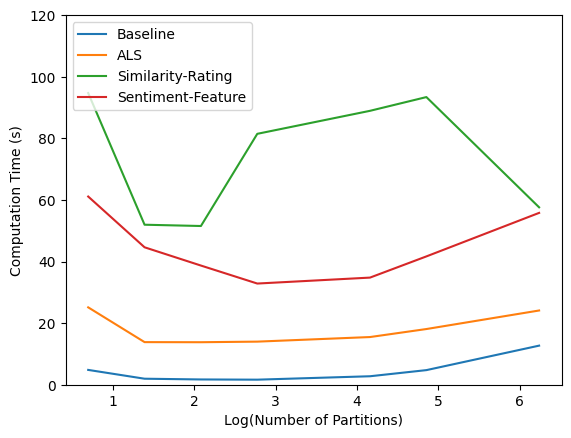
\includegraphics[width=0.4\textwidth]{partition_magazine_graph.png}
\end{figure}

\begin{figure}[h]
\caption{Computation Time for Different Models and Partitions on Luxury Dataset}
\centering
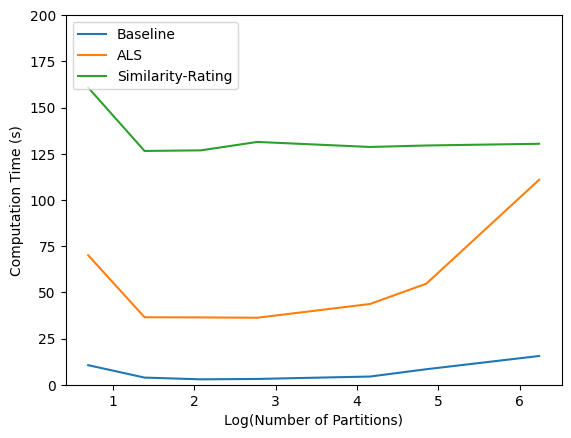
\includegraphics[width=0.4\textwidth]{partition_luxury_graph.png}
\end{figure}

There is a clear distinction in computation time across models across all partitions observed in the results for the data partitioning trials. The baseline model is significantly faster than ALS, and ALS is faster than the Similarity-Rating model across both datasets. A faster computation time was also observed for Sentiment-Feature compared to Similarity-Rating on the magazine dataset. This is interesting given the troubles we had with running the Sentiment-Feature model on a larger dataset. However, we have also observed that run times on the Google Cloud Platform can fluctuate across different runs even with the same settings, potentially caused by changes in resource availability on the platform. Thus it is hard to conclusively say that the Similarity-Rating model is always slower than the Sentiment-Feature model.   

Furthermore, it is observed that increasing the number of partitions leads to a decrease in the computation time up to a certain partition setting. Increasing the number of partitions beyond this optimum setting leads to an increase in the computation time for most models. This indicates that too few or too many partitions generally increase the computation time. This was consistently observed for the baseline and ALS model across the two datasets, and also for the Sentiment-Features model in the smaller magazine dataset. 

However, the relationship between computation time and partition for the similarity rating model is slightly different across both datasets. On the magazine dataset, the above common pattern was observed up until partition size of 128, but we see a computation time increase again when partition size increases to 512. We suspect this is due to the fluctuations in resource availability on the google cloud platform, and may require further investigation. Performance on the luxury dataset does not show the typical increase in computation time as partitions increase, suggesting similarity-rating may be more robust to partitioning than other models. 

In addition, it is observed that the performance results for both the baseline and ALS model remain the same across partitions up until four decimal places, while there are some small fluctuations in the results across partitions for the Similarity-Rating model and Sentiment-Feature model. This indicates that throughout the process of repartitioning, the Similarity-Rating model and Sentiment-Feature model are less robust against re-distributing data, such that when the results were compiled together they fluctuate more across runs. Nevertheless, the fluctuations are not extremely significant and still allow for good cross-model comparisons.

Finally, comparing across the two datasets, it appears that the optimal number of partitions remains roughly the same across the baseline models despite one dataset being 6 times the size of the other. The optimal number seems to be around 8/16 for both. The optimal partition for the Sentiment-Feature model is also 16 for the Magazine dataset, although the increase in computation time from further partition increases seems less sharp than that of the baseline models. The optimal partition remains more ambiguous for the Similarity-Rating model. 

\begin{table}
        \caption{Computational Time Across Models \& Partitions for Magazine Dataset}
        \label{tab:compute_magazine}
        \begin{tabular}{@{}cccccc@{}}
        \toprule
        \textbf{Model} & \textbf{Partition} & \textbf{MSE} & \textbf{RMSE} & \textbf{MAE} & \textbf{Time(s)} \\
        \midrule
        \multirow{7}{*}{Baseline} & 2 & 1.8083 & 1.3447 & 1.0141 & 4.8079 \\
                 & 4 & 1.8083 & 1.3447 & 1.0141 & 1.9474 \\
                 & 8 & 1.8083 & 1.3447 & 1.0141 & 1.7147 \\
                 & 16 & 1.8083 & 1.3447 & 1.0141 & 1.6411 \\
                 & 64 & 1.8083 & 1.3447 & 1.0141 & 2.7514 \\
                 & 128 & 1.8083 & 1.3447 & 1.0141 & 4.7375 \\
                 & 512 & 1.8083 & 1.3447 & 1.0141 & 12.6944 \\\midrule
        \multirow{7}{*}{ALS} & 2 & 4.0593 & 2.0148 & 1.6717 & 25.1188 \\
                 & 4 & 4.0593 & 2.0148 & 1.6717 & 13.8272 \\
                 & 8 & 4.0593 & 2.0148 & 1.6717 & 13.8005 \\
                 & 16 & 4.0593 & 2.0148 & 1.6717 & 13.9936 \\
                 & 64 & 4.0593 & 2.0148 & 1.6717 & 15.4770 \\
                 & 128 & 4.0593 & 2.0148 & 1.6717 & 18.0805 \\
                 & 512 & 4.0593 & 2.0148 & 1.6717 & 24.0991 \\\midrule
        \multirow{7}{*}{Similarity-Rating} & 2 & 1.9140 & 1.3835 & 1.0216 & 94.6977 \\
                 & 4 & 1.9109 & 1.3823 & 1.0215 & 51.9459 \\
                 & 8 & 1.9138 & 1.3834 & 1.0218 & 51.5331 \\
                 & 16 & 1.9100 & 1.3820 & 1.0209 & 81.4571 \\
                 & 64 & 1.9119 & 1.3827 & 1.0212 & 88.9344 \\
                 & 128 & 1.9105 & 1.3822 & 1.0209 & 93.3863 \\
                 & 512 & 1.9113 & 1.3825 & 1.0216 & 57.5985 \\\midrule
        \multirow{7}{*}{Sentiment-Feature} & 2 & 2.8168 & 1.6783 & 1.5218 & 61.10 \\
                 & 4 & 2.8141 & 1.6775 & 1.5206 & 44.6204 \\
                 & 8 & 2.8144 & 1.6776 & 1.5211 & 38.6916 \\
                 & 16 & 2.8145 & 1.6777 & 1.5214 & 32.8457 \\
                 & 64 & 2.8148 & 1.6777 & 1.5212 & 34.7765 \\
                 & 128 & 2.8138 & 1.6775 & 1.5212 & 41.6569 \\
                 & 512 & 2.8168 & 1.6783 & 1.5218 & 55.7854 \\
        \bottomrule
        \end{tabular}
    \end{table}

\begin{table}
        \caption{Computational Time Across Models \& Partitions for Luxury Dataset}
        \label{tab:compute_luxury}
        \begin{tabular}{@{}cccccc@{}}
        \toprule
        \textbf{Model} & \textbf{Partition} & \textbf{MSE} & \textbf{RMSE} & \textbf{MAE} & \textbf{Time(s)}  \\
        \midrule
        \multirow{7}{*}{Baseline} & 2 & 1.4900 & 1.2207 & 0.8618 & 10.5751 \\
                 & 4 & 1.4900 & 1.2207 & 0.8618 & 3.8614 \\
                 & 8 & 1.4900 & 1.2207 & 0.8618 & 2.9239 \\
                 & 16 & 1.4900 & 1.2207 & 0.8618 & 3.1289 \\
                 & 64 & 1.4900 & 1.2207 & 0.8618 & 4.4292 \\
                 & 128 & 1.4900 & 1.2207 & 0.8618 & 8.3907 \\
                 & 512 & 1.4900 & 1.2207 & 0.8618 & 15.5540 \\\midrule
        \multirow{7}{*}{ALS} & 2 & 3.6699 & 1.9157 & 1.6055 & 70.0459 \\
                 & 4 & 3.6699 & 1.9157 & 1.6055 & 36.5092 \\
                 & 8 & 3.6699 & 1.9157 & 1.6055 & 36.4170 \\
                 & 16 & 3.6699 & 1.9157 & 1.6055 & 36.2411 \\
                 & 64 & 3.6699 & 1.9157 & 1.6055 & 43.6892 \\
                 & 128 & 3.6699 & 1.9157 & 1.6055 & 54.6916 \\
                 & 512 & 3.6699 & 1.9157 & 1.6055 & 110.8976 \\\midrule
        \multirow{7}{*}{Similarity-Rating} & 2 & 1.5871 & 1.2598 & 0.8862 & 160.7877 \\
                 & 4 & 1.5842 & 1.2586 & 0.8850 & 126.4920 \\
                 & 8 & 1.5831 & 1.2582 & 0.8847 & 126.8321 \\
                 & 16 & 1.5860 & 1.2594 & 0.8859 & 131.3768 \\
                 & 64 & 1.5866 & 1.2592 & 0.8854 & 128.6622 \\
                 & 128 & 1.5855 & 1.2592 &  0.8854 & 129.4615 \\
                 & 512 & 1.5845 & 1.2588 & 0.8851 & 130.3827 \\
        \bottomrule
        \end{tabular}
    \end{table}
    


\section{Conclusion}

The conclusion of the project can be summarised by our findings regarding the two main investigative focuses. Firstly, the best model on average across the 18 Amazon review datasets investigated is the Baseline Rating Model, followed closely by the Similarity-Rating Model. The ALS and Sentiment-Feature model performed quite a bit worse than these two models, with the ALS having better MAE while the Similarity-Rating has better mean squared errors. We believe the results are informative but they should be judged against how the two customer-reviews-based models were designed to be a model with general settings, and think that the two customer-reviews-based models have the potential for improvements. Secondly, it is observed that increasing the number of partitions leads to a decrease in the computation time up to a certain partition setting. Increasing the number of partitions beyond this optimum setting leads to an increase in the computation time for most models. Computation time is fastest for Baseline Rating Model across all partition settings, followed by ALS, Sentiment-Feature and Similarity-Rating. We believe our work can act as a reference for further work in investigating how customer reviews can be utilised to make better rating predictions and thus better product recommender systems. 
 
A key limitation of this report was time and computational resources, given the one-month scope of the project and the limited Google Cloud credits available. Thus, we propose the following extensions to this report. First, both the Similarity-Rating and Sentiment-Feature models can be further developed and optimised for the Amazon reviews dataset, such as by training hyperparameters, and exploring more sophisticated ways of combining results rather than taking the average. Second, while we have demonstrated the impact of increasing partitions on computing performance, more distributed computing trials can be done on further increasing memory or changing the number of worker nodes, which could be used to inform further scaling up of the models. Furthermore, similar distributed methods and approaches as those suggested in this report can be explored for applying a topic modelling model such as LDA for building a customer-reviews-based recommender system, which was not covered within the scope of this project. 

\bibliographystyle{ACM-Reference-Format}
\bibliography{bibliography}

\section{Statement}
All students contributed equally to the technical aspects of this study. 52208 worked on the ALS model and the Sentiment Model. 44326 worked on the Baseline Model, the Similarity Model and the Sentiment Model. 42193 worked on the ALS model and the Sentiment Model. All students worked on Apache Hadoop and Apache Spark to scale the models to work on large datasets. 
\appendix
\section{Complete Table}
The complete table of matrices that evaluates the performance of models using all per-category data is shown on the next page.
    \begin{table*}
        \caption{Performance of Models, All Categories}
        \label{tab:perform}
        \begin{tabular}{cccccc}
        
        \toprule
        \textbf{Dataset} & \textbf{Model} & \textbf{MSE} & \textbf{RMSE} & \textbf{MAE} \\ \midrule
        \multirow{4}{*}{All Beauty} & Baseline & 1.717823 & 1.310657 & 0.974093 \\
         & ALS & 5.847922 & 2.418248 & 2.097802 \\
         & Similarity & 1.77769 & 1.3333 & 1.011797 \\
         & Sentiment\footnote[1] & 2.934868 & 1.713145 & 1.5826820 \\ \midrule
        \multirow{4}{*}{Amazon Fashion} & Baseline & 2.022984 & 1.422317 & 1.080362 \\
         & ALS & 6.176146 & 2.485185 & 2.145212 \\
         & Similarity & 2.029906 & 1.424748 & 1.086842 \\
         & Sentiment\footnote[1] & 2.760515 & 1.661480 & 1.511704 \\ \midrule
        \multirow{4}{*}{Appliances} & Baseline & 1.577673 & 1.256054 & 0.880798 \\
         & ALS & 4.3724 & 2.091028 & 1.763048 \\
         & Similarity & 1.735171 & 1.317259 & 0.997394 \\
         & Sentiment\footnote[1] & 3.247280 & 1.802021 & 1.718007 \\ \midrule
        \multirow{4}{*}{Arts Crafts and Sewing} & Baseline & 1.441867 & 1.200778 & 0.822822 \\
         & ALS & 2.836493 & 1.684189 & 1.347271 \\
         & Similarity & 1.584661 & 1.258833 & 0.824249 \\
         & Sentiment\footnote[1] & 3.126371 & 1.768154 & 1.659531 \\ \midrule
        \multirow{4}{*}{CDs and Vinyl} & Baseline & 0.98714 & 0.993549 & 0.659377 \\
         & ALS & 1.881561 & 1.3717 & 1.07855 \\
         & Similarity & 1.306053 & 1.142827 & 0.743871 \\
         & Sentiment\footnote[1]& 3.220199 & 1.794491 & 1.70232 \\ \midrule
        \multirow{4}{*}{Digital Music} & Baseline & 0.737282 & 0.858651 & 0.494056 \\
         & ALS & 2.546375 & 1.595737 & 1.237013 \\
         & Similarity & 0.799045 & 0.893893 & 0.335644 \\
         & Sentiment\footnote[1] & 3.220199 & 1.794491 & 1.70232 \\ \midrule
        \multirow{4}{*}{Grocery and Gourmet Food} & Baseline & 1.566025 & 1.251409 & 0.856292 \\
         & ALS & 2.796861 & 1.672382 & 1.352853 \\
         & Similarity & 1.816373 & 1.347729 & 0.881575 \\
         & Sentiment \footnote[1]& 3.13973 & 1.771928 & 1.663404 \\ \midrule
        \multirow{4}{*}{Industrial and Scientific} & Baseline & 1.545425 & 1.243151 & 0.866539 \\
         & ALS & 3.40411 & 1.845023 & 1.514613 \\
         & Similarity & 1.647732 & 1.28364 & 0.912473 \\
         & Sentiment\footnote[1] & 3.051861 & 1.746957 & 1.633147 \\ \midrule
        \multirow{4}{*}{Kindle Store} & Baseline & 1.099818 & 1.048722 & 0.731406 \\
         & ALS & 2.306926 & 1.518857 & 1.211931 \\
         & Similarity & 1.338263837 & 1.156833539 & 0.7682287502 \\
         & Sentiment\footnote[1] & 2.726755 & 1.651289 & 1.501492 \\ \midrule
        \multirow{4}{*}{Luxury Beauty} & Baseline & 1.500002 & 1.224746 & 0.865413 \\
         & ALS & 3.723059 & 1.929523 & 1.623528 \\
         & Similarity & 1.596616 & 1.263573 & 0.889901 \\
         & Sentiment\footnote[1] & 2.959361 & 1.720279 & 1.588605 \\ \midrule
        \multirow{4}{*}{Magazine Subscriptions} & Baseline & 1.808252 & 1.344713 & 1.014084 \\
         & ALS & 4.059702 & 2.01487 & 1.671833 \\
         & Similarity & 1.910562 & 1.382231 & 1.019775 \\
         & Sentiment & 2.789892 & 1.670297 & 1.511729 \\ \midrule
         \multicolumn{5}{r}{Continued on next page} \\ \bottomrule

        \end{tabular}
    \end{table*}

         
    \begin{table*}
    \ContinuedFloat
        \caption{Performance of Models, All Categories (Continued)}
        \label{tab:perform}
        \begin{tabular}{cccccc}
        
        \toprule
        \textbf{Dataset} & \textbf{Model} & \textbf{MSE} & \textbf{RMSE} & \textbf{MAE} \\ \midrule
        \multirow{4}{*}{Musical Instruments} & Baseline & 1.533344 & 1.238283 & 0.875227 \\
         & ALS & 3.019845 & 1.73777 & 1.412391 \\
         & Similarity & 1.705711 & 1.306029 & 0.887728 \\
         & Sentiment\footnote[1] & 2.991674 & 1.729645 & 1.609481 \\ \midrule
         \multirow{4}{*}{Office Products} & Baseline & 1.700172 & 1.303906 & 0.932472 \\
         & ALS & 3.273364 & 1.809244 & 1.475265 \\
         & Similarity & 1.924311 & 1.387195 & 0.936604 \\
         & Sentiment\footnote[1] & 3.090192 & 1.757894 & 1.652454 \\ \midrule
        \multirow{4}{*}{Patio Lawn and Garden} & Baseline & 1.842985 & 1.357566 & 0.986005 \\
         & ALS & 3.438762 & 1.85439 & 1.530015 \\
         & Similarity & 2.149091 & 1.465978 & 0.996309 \\
         & Sentiment\footnote[1] & 3.056682 & 1.748337 & 1.639639 \\ \midrule
        \multirow{4}{*}{Pet Supplies} & Baseline & 1.747074 & 1.321769 & 0.955178 \\
         & ALS & 3.0014 & 1.732455 & 1.428014 \\
         & Similarity & 2.221644 & 1.490518 & 0.985505 \\
         & Sentiment\footnote[1] & 2.934268 & 1.71297 & 1.582691 \\ \midrule
        \multirow{4}{*}{Prime Pantry} & Baseline & 1.313581 & 1.146116 & 0.781451 \\
         & ALS & 2.40808 & 1.551799 & 1.221744 \\
         & Similarity & 1.548462 & 1.244372 & 0.803368 \\
         & Sentiment\footnote[1] & 3.094914 & 1.759236 & 1.650479 \\ \midrule
        \multirow{4}{*}{Software} & Baseline & 2.401111 & 1.549552 & 1.256019 \\
         & ALS & 5.269411 & 2.29552 & 1.940394 \\
         & Similarity & 2.795662 & 1.672023 & 1.262217 \\
         & Sentiment\footnote[1] & 2.95417 & 1.71877 & 1.590463 \\ \midrule
        \multirow{4}{*}{Video Games} & Baseline & 1.855148 & 1.362038 & 1.017841 \\
         & ALS & 3.503129 & 1.871665 & 1.542054 \\
         & Similarity & 2.191238 & 1.480283 & 1.028966 \\
         & Sentiment\footnote[1] & 2.917326 & 1.708018 & 1.574277 \\ \midrule
         \multicolumn{5}{l}{\footnote[1]NThe result was run on a subset of the first 10,000 observations of the dataset.} \\ \bottomrule
        \end{tabular}
    \end{table*}

\end{document}